\documentclass{standalone}
\usepackage{tikz}
\usepackage{amsmath}

\definecolor{mygreen}{RGB}{117,167,117}
\definecolor{myred}{RGB}{255,1,1}

\newcommand\myent[1]{%
  \footnotesize%
  $#1$
}

\begin{document}

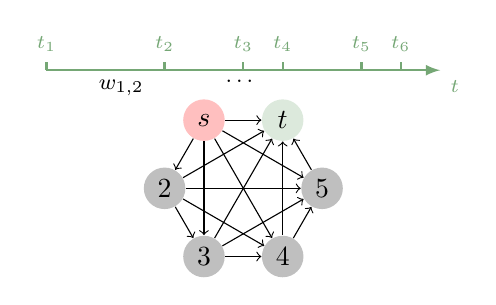
\begin{tikzpicture}[x=0.5cm]
  \draw[mygreen,->,thick,>=latex] (0,0) -- (10,0) node[below right] {$\scriptstyle t$};

  \draw[mygreen,thick] (0,0) -- ++(0,3pt) node[above] {$\scriptstyle t_1$};
  \draw[mygreen,thick] (3,0) -- ++(0,3pt) node[above](center1) {$\scriptstyle t_2$};
  \draw[mygreen,thick] (5,0) -- ++(0,3pt) node[above] {$\scriptstyle t_3$};
  \draw[mygreen,thick] (6,0) -- ++(0,3pt) node[above] {$\scriptstyle t_4$};
  \draw[mygreen,thick] (8,0) -- ++(0,3pt) node[above] {$\scriptstyle t_5$};
  \draw[mygreen,thick] (9,0) -- ++(0,3pt) node[above] {$\scriptstyle t_6$};
  
  
  \node[below,align=left,anchor=north,inner xsep=0pt] at (2,0) {\myent{w_{1,2}}};  
  \node[below,align=left,anchor=north,inner xsep=0pt] at (5,0) {\myent{\ldots}};  

  \tikzstyle{vertex}=[circle,fill=black!25,minimum size=15pt,inner sep=0pt]
  \tikzstyle{svertex}=[circle,fill=red!25,minimum size=15pt,inner sep=0pt]
  \tikzstyle{tvertex}=[circle,fill=mygreen!25,minimum size=15pt,inner sep=0pt]
  
%   \path (center1.south)+(1.5, 0) 
%   	node (Q-1) [svertex,xshift=9cm,yshift=.5cm] at (120:1cm) {$s$};
  \def \centerx{2.5cm}
  \def \centery{-1.5cm}
  
  \node[svertex,xshift=\centerx, yshift=\centery] (Q-1) at (120:1cm) {$s$};
  \node[tvertex,xshift=\centerx,yshift=\centery] (Q-6) at (60:1cm) {$t$};
  
  \foreach \name/\angle/\text in {Q-2/180/2, Q-3/240/3, Q-4/-60/4, Q-5/0/5}
	\node[vertex,xshift=\centerx,yshift=\centery] (\name) at (\angle:1cm) {$\text$};

  \foreach \from/\to in {1/2,1/3,1/4,1/5,1/6,2/3,2/4,2/5,2/6,3/4,3/5,3/6,4/5,4/6,5/6}
  	\path [draw, ->] (Q-\from) -- (Q-\to);
    
\end{tikzpicture}
\end{document}



% \begin{document}
% \pagestyle{empty}
% \begin{tikzpicture}[shorten >=1pt,->]

% 	\tikzstyle{vertex}=[circle,fill=black!25,minimum size=17pt,inner sep=0pt]
    
%     \foreach \name/\x in {s/1, 2/2, 3/3, 4/4, 15/11, 16/12, 17/13, 18/14, 19/15, t/16}
% 		\node[vertex] (G-\name) at (\x,0) {$\name$};

%     \foreach \name/\angle/\text in {P-1/234/5, P-2/162/6,P-3/90/7, P-4/18/8, P-5/-54/9}
% 		\node[vertex,xshift=6cm,yshift=.5cm] (\name) at (\angle:1cm) {$\text$};

% 	\foreach \name/\angle/\text in {Q-1/234/10, Q-2/162/11, Q-3/90/12, Q-4/18/13, Q-5/-54/14}
%       	\node[vertex,xshift=9cm,yshift=.5cm] (\name) at (\angle:1cm) {$\text$};

% 	\foreach \from/\to in {s/2,2/3,3/4,3/4,15/16,16/17,17/18,18/19,19/t}
% 		\draw (G-\from) -- (G-\to);

% 	\foreach \from/\to in {1/2,2/3,3/4,4/5,5/1,1/3,2/4,3/5,4/1,5/2}
% 	{ \draw (P-\from) -- (P-\to); \draw (Q-\from) -- (Q-\to); }

%     \draw (G-3) .. controls +(-30:2cm) and +(-150:1cm) .. (Q-1);
%     \draw (Q-5) -- (G-15);
% \end{tikzpicture}
% \end{document}